\chapter{The Standard Model of Particle Physics }
\epigraph{\itshape Barrabas came to us by sea, the child Clara wrote in her delicate calligraphy.}{Isabel Allende, \textit{The House of the Spirits} }

\linenumbers

Particle physics studies the fundamental interactions of the universe. Everything from the nuclear interactions occurring in the center of stars to simple electron interactions. The Standard Model is currently the best tool for achieving this goal. This model is the result of combined efforts from generations of physicists; it encapsulates centuries of experimental results and is the most accurate scientific model to date.

The Standard Model consists of three generations of quarks and leptons (fermions) along with 5 physically manifesting bosons. Leptons consist of electrons, muons, taus, and three neutrinos. The quarks are fractionally charged particles which are observed in bound states called hadrons. The bosons are mediators of interactions; a number of bosons are present in the Standard Model, 5 of which manifest at our energy scales.

Group theory is the language of the standard model and requires some mathematical introduction

\section{Mathematical Introduction}

Physics aims to describe our universe mathematically. Frequently, this requires describing how objects behave under transformations. The mathematical study of this behavior is called Group Theory. It is one of the greatest mathematical achievements--providing underlying structures used in physics, materials science, and chemistry. For particle physics, it is crucial to have a basic understanding of several important groups and definitions \cite{GroupTheoryBook}.

The Standard Model is built on the unitary group and its special unitary subgroup. A unitary group $U(n)$ is defined as:

\newtheorem{theorem}{Theorem}[section]
\newtheorem{definition}[theorem]{Definition}

\begin{definition}
$U(n)$ is the group of all $n \times n$ matrices, $T$, such that $T^{-1}=T^{\dagger}$  
\end{definition}
In other words, $U(n)$ is the group of all unitary $n \times n$ matrices. It has an important subgroup called the special unitary group $SU(n)$.

\begin{definition}
$SU(n)$ is the group of all $T \in U(n)$ such that $\det(T) =1$.
\end{definition}
$U(n)$ and $SU(n)$ are both examples of Lie groups. Lie groups represent a large field of study in mathematics; many thorough texts exist on the subject and a complete definition requires a large mathematical background. However, the Standard Model is limited to matrix Lie groups. 

\begin{definition}
A matrix Lie group is a group of invertible $n\times n$ matrices on $\mathbb{R}$ or $\mathbb{C}$.
\end{definition}
This structure allows for a mathematical description of continuous motions and thus symmetries in physics \cite{GroupTheoryBook}.

Each Lie group has a corresponding Lie algebra

\begin{definition}
Let $G$ be a matrix Lie group. Then, the Lie algebra is the set of all matrices $X$ such that $e^{tX}\in G$ for all real numbers $t$.
\end{definition}
The Lie algebra may be thought of as the elements that are infinitesimally close to the identity in a Lie group. In physics, these elements are called generators and describe infinitesimal transformations. Generators become particularly important when used in representation theory \cite{GroupTheoryBook}.

Representation theory formalizes the language of transformations in physics.

\begin{definition}
Let $G$ be a matrix Lie group, $V$ be a vector space, and $g\in G$. Consider a map $\phi$ such that $\phi : g \rightarrow X$ where $X$ is a linear operator on $V$. Together, $\phi$ and $V$ are called a representation.
\end{definition}
A representation takes a group element and maps it to a linear operator on a vector space. When the representations of the generators are exponentiated, they describe finite transformations (i.e. the Lie group elements). Thus, objects in physics are vectors in a vector space, transformations of objects are linear operators that act on those vectors, and generators are used to construct those linear operators \cite{GroupTheoryBook, Peskin}. This language of transformations makes it possible to mathematically describe particle interactions.


\section{The Standard Model Gauge Group} 

Centuries of experiments have led to the observation of symmetries in nature. The observed symmetries of the universe are embedded in our Physical models. Mathematically, this is accomplished with various gauge groups. Some of these symmetries are only present at a high energy scale and manifest differently at non-extreme energies--these are called "broken" symmetries. The Standard Model is described mathematically by the gauge group $SU(3)\times SU(2) \times U(1)$ and utilizes both broken and unbroken symmetries \cite{Langacker}.

Quantum Chromodynamics (QCD) is the theory of strong interactions and is described by $SU(3)$, an unbroken symmetry. This $SU(3)$ theory yields three types of charge called "colour" and describes how quarks interact and bind together into hadrons.

$SU(2)\times U(1)$ describes the electroweak interaction and unlike QCD is a broken symmetry. This broken symmetry is at the heart of the standard model, it describes the electroweak force at high values of energy and breaks into two separate forces at the low energy scales we observe in our daily lives. In fact, this clever theory happens to break in exactly the right way to explain all electroweak observations to date \cite{Griffiths}.

\section{Electroweak Theory}

In 1961, Glashow proposed the idea of using $SU(2)\times U(1)$ to describe electroweak interactions \cite{Glashow}. But there was a problem! This theory required that the bosons mediating the electroweak interactions were massless, which disagreed with experimental observations of weak interactions. Then in 1964, Higgs, Brout, and Englert proposed a method for spontaneous symmetry breaking by introducing a scalar field with a non-zero vacuum expectation value. The field became known as the "Higgs field" and this method became known as the "Higgs mechanism" \cite{BroutEnglert, Higgs}. This theoretical breakthrough finally provided an explanation for massive bosons. But the Higgs mechanism is even more encompassing than that, it provides an explanation for the origin of mass in the standard model.

In the late 1960s Weinberg and Salam used the Higgs mechanism to describe electroweak symmetry breaking. Thus, describing low energy electromagnetic interactions with the massless photon and weak interactions with the massive W and Z bosons \cite{Weinberg, Salam}. The resulting theory has incredible experimental agreement--encompassing centuries of results and successfully predicting many observations. Because of this success, Glashow, Salam, and Weinberg were awarded the noble prize in 1979 for electroweak unification. 

The Glashow-Salam-Weinberg (GSW) theory consists of three stages during the evolution of the universe: 
\begin{itemize}
    \item The high energy electroweak interaction (i.e. during the early universe).
    \item The spontaneous symmetry breaking that occurs via the Higgs mechanism as the universe cools.
    \item The resulting low energy electromagnetic and weak interactions (i.e. the present day).
\end{itemize}

\subsection{The High Energy Electroweak Interaction}

To start understanding this theory, consider the period of time immediately after the Big Bang. In GSW theory, the very early universe ($t<10^{-12}$ s) existed at temperatures greater than $10^{16}$ K where there was one electroweak interaction. In this early universe, the Higgs field existed in an excited state so all of the fermions were massless. These electroweak interactions are described by the kinetic terms in Eq.~\ref{noMassLag} \cite{Blundell, Peskin}.
\begin{equation}
    \mathcal{L} = \bar{E}_{L}(i\cancel{D})E_{L}+ \bar{e}_{R}(i\cancel{D})e_{R}+ \bar{Q}_{L}(i\cancel{D})Q_{L}+ \bar{u}_{R}(i\cancel{D})u_{R}+ \bar{d}_{R}(i\cancel{D})d_{R}
    \label{noMassLag}
\end{equation}
In this Lagrangian, there are two important things to disentangle: the covariant derivative and the fermion fields. First, consider the covariant derivative for a $SU(2)$ fermion field
\begin{equation}
    D_{\mu}= \partial_{\mu} - igA^{a}_{\mu}\tau^{a}-ig'YB_{\mu} 
    \label{covDer}
\end{equation}
$Y$ represents the $U(1)$ charge called weak hypercharge and $\tau^{a}$ are the generators of $SU(2)$. The $\tau^{a}$ are the normalized Pauli matrices, $\tau^{a}=\frac{1}{2}\sigma^{a}$, where the eigenvalue, $T^{3}$, of the $\tau^{3}$ operator is called the weak isospin. $A^{a}_{\mu}$ and $B_{\mu}$ are the $SU(2)$ and $U(1)$ gauge bosons with coupling constants $g$ and $g'$. These massless bosons are called Goldstone bosons.

Fermions are chiral particles, meaning that the left- and right-handed fermions are two different representations of the same $SU(2)$ gauge group. In Eq.~\ref{noMassLag}, the L and R subscripts denote the left-handed and right-handed fermion fields. The left-handed fields are represented as doublets of $SU(2)$ and the right-handed fields are singlets of $SU(2)$ \cite{Peskin}

\begin{equation}
    E_{L} = \begin{pmatrix}
            \nu_{e}\\
            e^{-}
            \end{pmatrix}_{L}
    \; \;
    Q_{L} = \begin{pmatrix}
            u \\
            d
            \end{pmatrix}_{L}
    \; \;
    e_{R}
    \; \;
    u_{R}
    \; \;
    d_{R}
\end{equation}

This interaction of massless fermions with massless Goldstone bosons is the high energy electroweak interaction.

\subsection{Spontaneous Symmetry Breaking via the Higgs Mechanism}

As the universe cooled below $10^{16}$ K, the Higgs field settled to a ground state with a non-zero vacuum expectation value and broke $SU(2) \times U(1)$ symmetry \cite{Blundell}. This relaxation of the Higgs field is shown in Fig.~\ref{fig:HiggsPotential}. The unique shape of the Higgs potential is key to the mass inducing symmetry breaking.

\begin{figure}[htb]
    \centering
    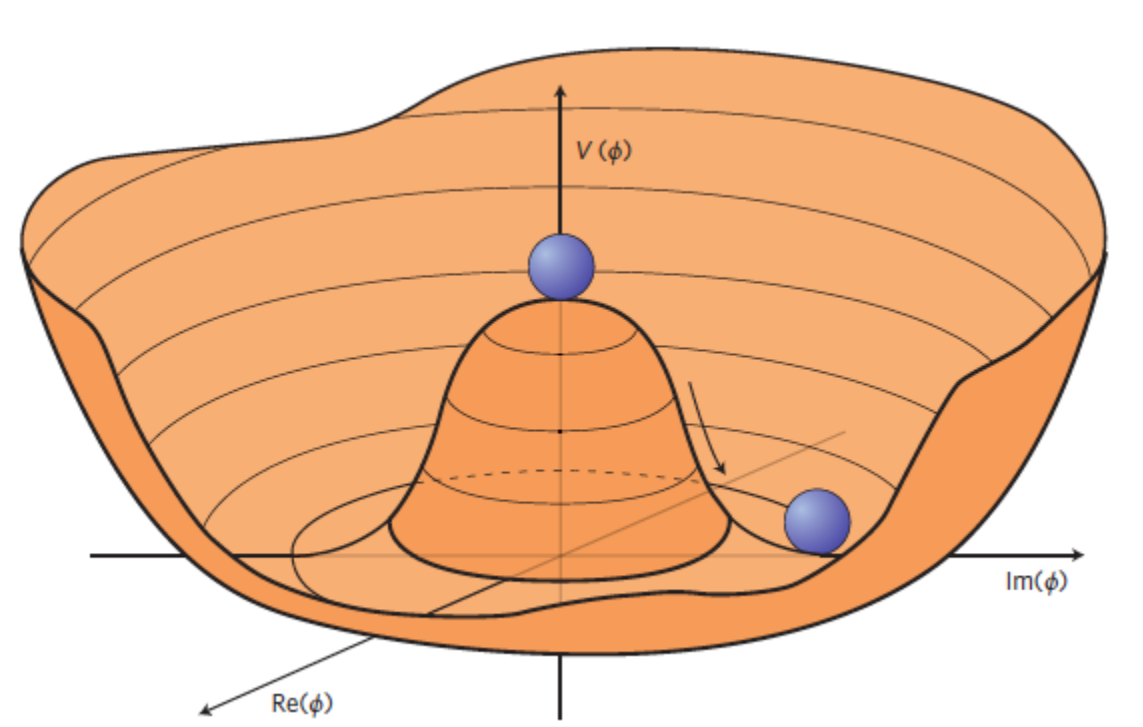
\includegraphics[width=8cm]{HiggsPotential.png}
    \caption{The Higgs potential with a non-zero vacuum expectation value. Figure from \cite{ellisHiggs}. }
    \label{fig:HiggsPotential}
\end{figure}

The Higgs field is a scalar field, $\phi$, that has a non-zero vacuum expectation value. One way of describing this field is by 
\begin{equation}
    \langle \phi \rangle = \frac{1}{\sqrt{2}}
    \begin{pmatrix}
    0 \\
    \nu
    \end{pmatrix}
\end{equation}
This scalar field undergoes the gauge transformation
\begin{equation}
    \phi \rightarrow e^{i\alpha^{a}\tau^{a}}e^{i\beta/2}\phi 
\end{equation}
with $\alpha^{1} = \alpha^{2} = 0$ and $\alpha^{3} = \beta$. Thus, $\langle \phi \rangle$ is invariant. This causes the emergence of one massless boson (the photon) and three massive bosons. The relevant terms for determining the masses are 
\begin{equation}
    \Delta \mathcal{L} = (D_{\mu}\phi)^{2} = \frac{1}{2}
    \begin{pmatrix}
    0 \; \nu
    \end{pmatrix}
    (g A^{a}_{\mu} \tau^{a} + \frac{1}{2}g'B_{\mu})(gA^{b\mu}\tau^{b}+\frac{1}{2}g'B^{\mu})
    \begin{pmatrix}
    0 \\
    \nu
    \end{pmatrix}
\end{equation}
which reduces to

\begin{equation}
    \Delta \mathcal{L} = \frac{1}{2}\frac{\nu^{2}}{4}[g^{2}(A^{1}_{\mu})^2+g^{2}(A^{2}_{\mu})^{2}+(-gA^{3}_{\mu} + g'B_{\mu})^{2}]
\end{equation}
This equation describes three massive vector bosons and the massless photon \cite{Peskin}. They are 

\begin{align}
    \textrm{ The W bosons } \; &W^{\pm}_{\mu}=\frac{1}{\sqrt{2}} (A^{1}_{\mu} \mp iA^{2}_{\mu}) \; &&\textrm{  with  } \; m_{W} = g\frac{\nu}{2} \\
    \textrm{ The Z boson } \; &Z^{0}_{\mu}= \frac{1}{\sqrt{g^{2}+g'^{2}}}(gA^{3}_{\mu} - g'B_{\mu}) \; &&\textrm{  with  } \; m_{Z} = (\sqrt{g^{2}+g'^{2}})\frac{\nu}{2} \\
    \textrm{ The photon } \; &A_{\mu}=\frac{1}{\sqrt{g^{2}+g'^{2}}}(g'A^{3}_{\mu}+gB_{\mu})
\end{align}

The universe cooled from a hot state with one electroweak interaction to the universe we know today with two interactions: electromagnetic and weak \cite{Peskin}. But what about the weak hypercharge and weak isospin? How are these quantities relevant to our observable quantities? 

To answer this question, let's return to Eq.~\ref{covDer}, the covariant derivative for a Fermion field. Using the eigenstates of the broken $SU(2) \times U(1)$ symmetry, the covariant derivative can be rewritten as
\begin{equation}
    D_{\mu}=\partial_{\mu}- i\frac{g}{\sqrt{2}}(W^{+}_{\mu}\tau^{+} + W^{-}_{\mu}T^{-}) - i \frac{1}{\sqrt{g^{2}+g'^{2}}}Z_{\mu}(g^{2}\tau^{3}-g'^{2}Y) + i\frac{gg'}{\sqrt{g^{2}+g'^{2} }}A_{\mu}(\tau^{3}+Y)
    \label{covDerMass}
\end{equation}
with $\tau^{\pm}=\tau^{1}\pm i\tau^{2}$. The last term in this covariant derivative corresponds to the electromagnetic interaction. From this term, the electron charge and corresponding quantum number can be identified
\begin{align}
    e = \frac{gg'}{\sqrt{g^{2}+g'^{2}}} \\
    Q = T^{3} + Y
\end{align}
Thus, the electric charge quantum number is the sum of weak isospin and weak hypercharge. Also, a new measurable parameter can be introduced called the Weinberg angle $\theta_{w}$. This angle is defined such that
\begin{align}
    cos \theta_{w} = \frac{g}{\sqrt{g^{2}+g'^{2}}} && sin \theta_{w} = \frac{g'}{\sqrt{g^{2} + g'^{2}}}
\end{align}
This allows the change of basis relating Eq.~\ref{covDer} to Eq.~\ref{covDerMass} to be written as
\begin{equation}
    \begin{pmatrix}
    Z^{0} \\
    A
    \end{pmatrix}
    =
    \begin{pmatrix}
    cos \theta_{w} & -sin \theta_{w} \\
    sin \theta_{w} & cos \theta_{w} \\
    \end{pmatrix}
    \begin{pmatrix}
    A^{3} \\
    B
    \end{pmatrix}
\end{equation}
and as a result

\begin{align}
    g = \frac{e}{sin \theta_{w}} \\
    m_{W}=m_{Z}cos \theta_{w}
\end{align}

This means that electroweak interactions can be written in terms of three measurable parameters: $e$, $\theta_{w}$, and $m_{w}$ \cite{Peskin}. The electron charge was first experimentally measured by Millikan's oil drop experiment in 1909 \cite{OilDrop}. The Weinberg angle has been measured from many different experimental observations, such as: neutrino-proton scattering, neutrino-electron scattering, and the Z branching ratio \cite{Peskin}. The measured value is $\theta_{w}=28.75^{\textrm{o}}$ \cite{Griffiths}. The last missing piece is the W boson mass which was measured at CERN (along with the Z boson) in 1983 at $m_{W}=82$ GeV. GSW theory predicts then that the Z mass should be $93.5$ GeV which is in good agreement with CERN's measured value of $92$ GeV \cite{Griffiths, WBoson, ZBoson}. Now, all of these parameters have been measured at even greater precision and continue to show good agreement with the theory.

\;

\noindent{\textbf{Fermion Masses}}

The Higgs mechanism was motivated by the need to include massive bosons in the standard model. But fermion chirality adds in some complications for accounting for fermion masses. The left- and right-handed fermions belong to different representations of $SU(2)$ preventing the addition of simple mass terms \cite{Peskin}. Once again, the Higgs mechanism provides a solution to this dilemma.

To gain an intuition for the fermion mass terms, consider a full field $\psi=\psi_{L}+\psi_{R}$ and the Dirac Lagrangian $\mathcal{L}=\bar{\psi}(\cancel{p}-m)\psi$. This results in

\begin{equation}
    \mathcal{L}=\bar{\psi}_{L}\cancel{p}\psi_{L} + \bar{\psi}_{R}\cancel{p}\psi_{R} + m(\bar{\psi}_{L}\psi_{R} + \bar{\psi}_{R}\psi_{L})
\end{equation}

The intuition here is that a mass term will be of the form $m(\bar{\psi_{L}}\psi_{R}+h.c.)$ \cite{Blundell}. Such a term arises from the interaction of the Higgs field with the fermion fields. Consider the interaction of Higgs field and the first generation leptons. This results in
\begin{align}
    \Delta\mathcal{L}_{e} &= -\lambda_{e}\bar{E}_{L} \cdot \phi e_{R} + h.c. \\
    &= -\frac{1}{\sqrt{2}}\lambda_{e}\nu\bar{e}_{L}e_{R} + h.c. + \dots 
\end{align}
where $\lambda_{e}$ is a new dimensionless coupling constant (the Yukawa coupling) and $\phi$ was replaced with the vacuum expectation value. Thus,
\begin{equation}
    m_{e}=\frac{1}{\sqrt{2}}\lambda_{e}\nu
\end{equation}
The electron mass is scaled by $\lambda_{e}$ allowing the electron mass to differ greatly from the vacuum expectation value. This same procedure applies to the other lepton generations, giving rise to the muon and tau masses \cite{Blundell}. However, it is important to note that in GSW theory (and the current standard model) the neutrinos are massless which is experimentally shown to be false by the observation of neutrino oscillations \cite{NeutrinoOscSupK, NeutrinoOscSNO}. Thus, neutrinos must obtain mass from something other than the Higgs field.

Quarks obtain mass in a similar way as electrons. Consider one generation of quarks and the interaction of these quark fields with the Higgs field
\begin{align}
    \Delta \mathcal{L} &= \lambda_{d}\bar{Q}_{L} \cdot \phi d_{R} - \lambda_{u}\epsilon^{ab}\bar{Q}_{La} \phi^{\dagger} u_{R} + h.c. \\
    &= -\frac{1}{\sqrt{2}}\lambda_{d}\nu \bar{d}_{L}d_{R} - \frac{1}{\sqrt{2}}\lambda_{u}\nu \bar{u}_{L}u_{R} + h.c. + \dots
\end{align}
Thus, the up and down quark masses are
\begin{align}
    m_{d}=\frac{1}{\sqrt{2}}\lambda_{d}\nu &&
    m_{u}=\frac{1}{\sqrt{2}}\lambda_{u}\nu
\end{align}
The other generations obtain mass in the same way. The quark masses, like the lepton masses, depend on a dimensionless coupling $\lambda_{i}$ allowing for the large difference in masses observed experimentally. $\lambda_{i}$ are the Yukawa couplings; it is important to note that they are arbitrary and non-minimal \cite{Peskin}. 


\subsection{Low Energy Electroweak Currents and Interactions}

The three generations of quarks allow for terms that mix generations. This is more easily seen by considering a basis for the quark fields that diagnolizes their Higgs couplings (i.e. the mass matrix). A change of basis is a unitary transformation, in this case
\begin{align}
    u^{i}_{L}=U^{ij}_{u}u_{L}^{'j} &&
    d^{i}_{L}=U^{ij}_{d}d_{L}^{'j}
\end{align}
where $u^{i}_{L}=(u_{L},\; c_{L},\; t_{L})$ and $d^{i}_{L}=(d_{L},\; s_{L},\; b_{L})$ are the quark fields in the original basis and $u_{L}^{'i}$ and $d_{L}^{'i}$ are the quark fields in the mass eigenstate. The $W$ current can be derived from the covariant derivative for a fermion field (Eq.~\ref{covDerMass}) and expressed in the new mass eigenstate
\begin{align}
    J_{W}^{\mu +}&=\frac{1}{\sqrt{2}}\bar{u}^{i}_{L}\gamma^{\mu} d^{i}_{L} \\
    &=\frac{1}{\sqrt{2}}\bar{u}_{L}^{'i}\gamma^{\mu} (U^{\dagger}_{u}U_{d})_{ij}d_{L}^{'j} \\
    &=\frac{1}{\sqrt{2}}\bar{u}_{L}^{'i}\gamma^{\mu} V_{ij} d_{L}^{'j}
\end{align}
The new unitary matrix $V$ is the Cabibbo-Kobayashi-Maskawa (CKM) matrix \cite{Peskin}.

The CKM matrix describes the flavour mixing of quarks mediated by the $W$ boson, it is expressed as
\begin{equation}
    V =
    \begin{pmatrix}
    V_{ud} && V_{us} && V_{ub} \\
    V_{cd} && V_{cs} && V_{cb} \\
    V_{td} && V_{ts} && V_{tb} 
    \end{pmatrix}
\end{equation}
The off-diagonal elements specify interactions that occur across generations \cite{CKM}.

In the case of leptons, there is no right-handed neutrino, therefore there are no tree level generation changing interactions. 

The $Z$ current can also be derived using Eq.~\ref{covDerMass} and is given by
\begin{align*}
    J^{\mu}_{Z} = \frac{1}{cos\theta_{w}}[&\bar{\nu}_{L}\gamma^{\mu} (\frac{1}{2}) \nu_{L} + \bar{e}_{L}\gamma^{\mu}(-\frac{1}{2}+sin^{2}\theta_{w})e_{L} + \bar{e}_{R}\gamma^{\mu}(sin^{2}\theta_{w})e_{R} \\
    &+ \bar{u}_{L}\gamma^{\mu}(\frac{1}{2}-\frac{2}{3}sin^{2}\theta_{w})u_{L} + \bar{u}_{R}\gamma^{\mu}(-\frac{2}{3}sin^{2}\theta_{w})u_{R} \\
    &+ \bar{d}_{L}\gamma^{\mu}(-\frac{1}{2}+\frac{1}{3}sin^{2}\theta_{w})d_{L} + \bar{d}_{R}\gamma^{\mu}(\frac{1}{3}sin^{2}\theta_{w})d_{R}]
\end{align*}
In this equation, the $Z$ boson has no flavour changing interactions \cite{Peskin}.

Finally, the photon interactions are described by the standard electromagnetic current which can again be derived using Eq.~\ref{covDerMass}
\begin{equation}
    J^{\mu}_{EM}=\bar{e}\gamma^{\mu}(-1)e + \bar{u}\gamma^{\mu}(+\frac{2}{3})u + \bar{d}\gamma^{\mu}(-\frac{1}{3})d
\end{equation}
The photon, also does not allow for any flavour changing interactions \cite{Peskin}

Therefore, in the standard model, flavour changing neutral currents do not occur at tree level and are suppressed.

%\subsection{Electroweak Interactions}

The emergence of mass terms for the W and Z bosons creates a potential that varies as $U(r)\propto e^{-M r}$. Thus, the weak force is a short range force that falls off at distances greater than $\frac{1}{M}$. It is the magnitude of these masses that creates a "weaker" force than the electromagnetic force \cite{Blundell}. 

Electrically charged weak currents only affect left-handed fermions\footnote{Often, the weak interaction is denoted as $SU_{L}(2)$}. Whereas electromagnetic currents affect both left- and right-handed fermions \cite{Griffiths}. 

Electromagnetic currents describe the interactions of electrically charged particles and are mediated by the neutral photon. These interactions must conserve fermion flavour and obey charge and parity symmetry. Examples of electromagnetic interactions include: electron-positron annhilation and electron-electron scattering \cite{Griffiths}.

Neutral weak interactions are mediated by the $Z$ boson. All interactions mediated by the photon can also be mediated by the $Z$ boson. The neutral neutrinos have weak isospin and weak hypercharge, so the $Z$ boson can mediate neutrino scattering and neutrino-antineutrino annhilation/production. Additionally, neutral weak interactions can violate parity symmetry, but conserve fermion flavour. The $Z$ boson is its own anti-particle, so it has no weak isospin and no weak hypercharge \cite{Griffiths}.

Electrically charged weak interactions are mediated by the $W$ boson and are the only flavour changing interactions in the standard model. Due to the lack of right-handed neutrinos \footnote{To date, no right-handed neutrinos have been observed. However, they have not been completely ruled out experimentally and may interact very rarely--suppressing lepton flavour changing interactions.}, electrically charged weak vertices with leptons cannot occur across generations \cite{Griffiths}. However, this is not true for quarks. The CKM matrix gives the allowed quark-$W$ vertices and these interactions can be visualized nicely in Fig.~\ref{fig:CKMvisual}.

\begin{figure}[htb]
    \centering
    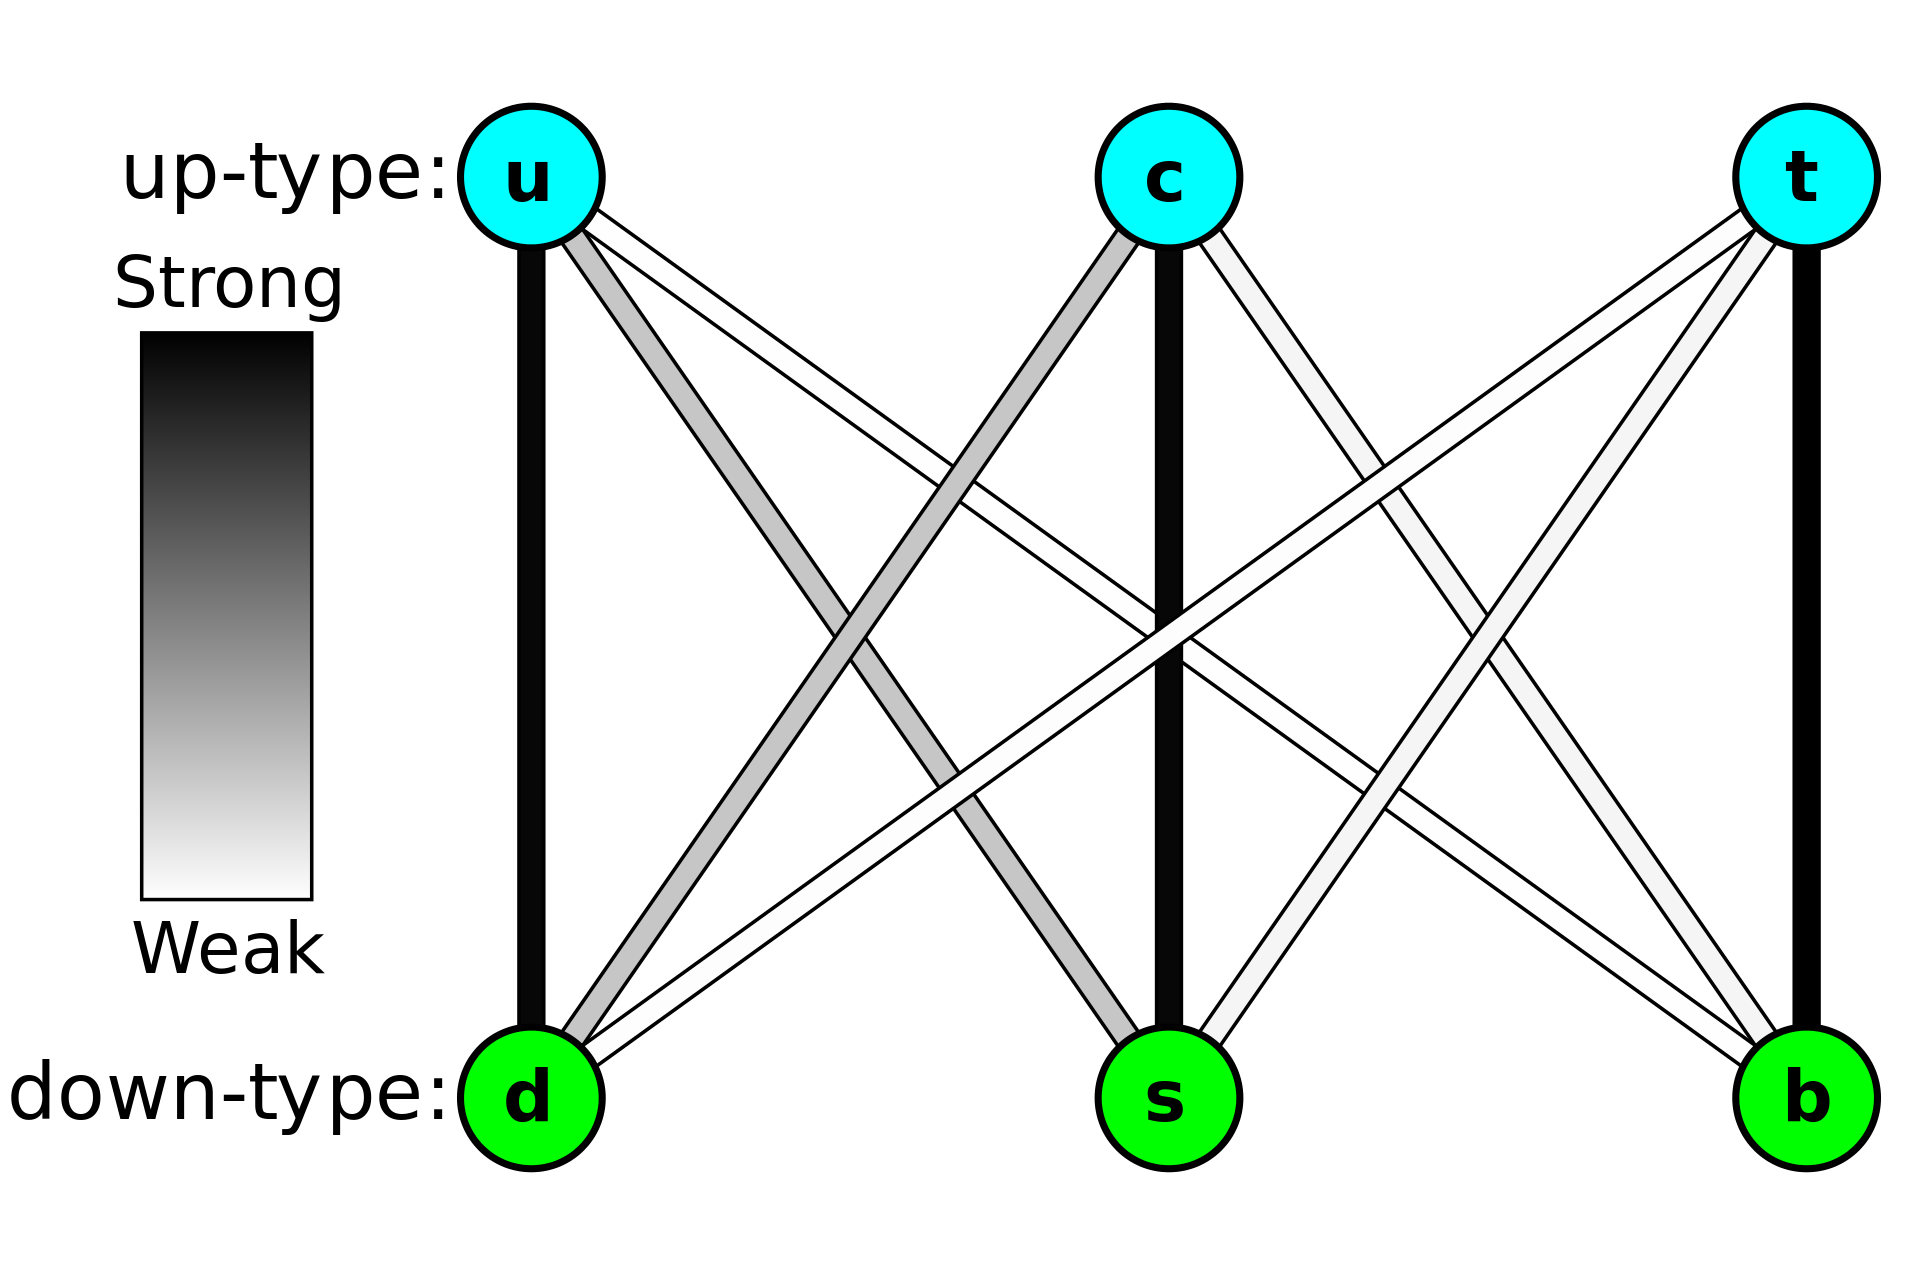
\includegraphics[width=8cm]{Quark_weak_interactions.png}
    \caption{The allowed quark-$W$ vertices. Figure from the public domain. }
    \label{fig:CKMvisual}
\end{figure}

There is a phase in the CKM matrix that allows these interactions to violate charge-parity symmetry, but charge-parity-time symmetry is still conserved. The $W$ boson carries weak isospin, but no weak hypercharge \cite{Griffiths}.

\subsection{The Higgs Boson}

The introduction of a scalar field with a non-zero vacuum expectation value has another consequence, it predicts the existence of a massive scalar boson, the Higgs boson. The mass of this new boson is given by
\begin{equation}
    m_{h}=\sqrt{\frac{\lambda}{2}}\nu
\end{equation}
which relies on a dimensionless constant $\lambda$ like the constants for the fermion masses \cite{Peskin}.

Interactions with the Higgs conserve flavour and the interaction strength defines the mass of the interacting particles. The Higgs boson is the only mediator that has weak hypercharge \cite{Peskin}.

The Higgs boson was discovered in 2012 at CERN with a mass of 125 GeV; it was the last standard model particle to be discovered \cite{HiggsBosonCMS, HiggsBosonATLAS}. Further measurements confirmed that the observed boson was indeed a scalar particle that coupled as predicted by the standard model \cite{PDGreview}. This further confirmed the predictions of the Standard Model.

\section{Beyond the Standard Model}

There are several notable issues with the standard model that motivate the need for a more complete theory. For example:
\begin{itemize}
\item In GSW theory the neutrinos are massless, which was proven false with the observation of neutrino oscillations \cite{NeutrinoOscSNO, NeutrinoOscSupK}. This means that neutrinos must obtain mass by some mechanism not explained in the standard model
\item Cosmological observations point to the existence of dark matter \cite{Griffiths, BulletCluster, GalaxyArm}. Such matter is not explained by any particle in the standard model.
\item One of the most common forces experienced in our daily lives, gravity, has no mediator in the standard model \cite{Peskin}.
\item Our universe is composed of matter rather than a mix of matter and anti-matter. A small asymmetry is explained by CP violation, but the large asymmetry seen in our universe is still unexplained \cite{Peskin, mattAsymmetry}.
\end{itemize}
These are some of the most commonly discussed short comings of the standard model. In addition to these observational issues, there are a number of theoretical problems; the most important for this thesis is the gauge hierarchy problem.

\subsection{Gauge Hierarchy Problem}
\label{gaugeHprob}

A hierarchy problem is created when divergent terms must be counteracted by introducing free parameters at a hierarchy of scales. 

\begin{figure}[htb]
    \centering
    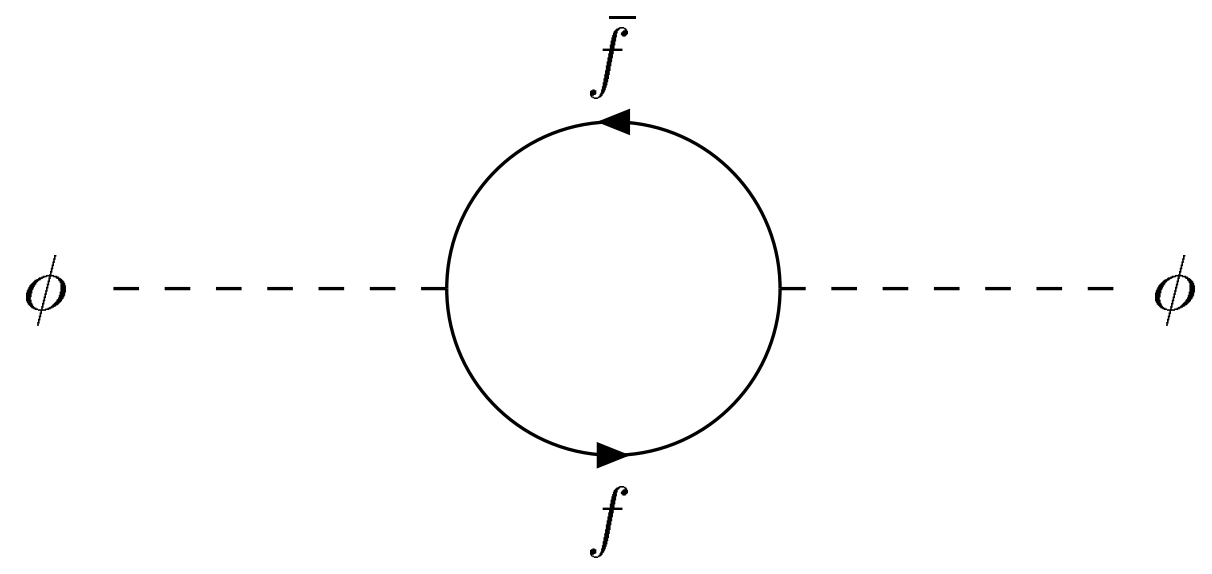
\includegraphics[width=7cm]{HiggsFermionSelfE.png}
    \caption{The fermion contribution to the Higgs self energy. Figure from \cite{SusyHiggsSelfE}}
    \label{HiggsSelfE}
\end{figure}

One such problem is caused by the the Higgs self energy. The fermion loop in Fig.~\ref{HiggsSelfE} contributes to the Higgs self energy with the corresponding equation
\begin{equation}
    \Sigma (0) = -2 N(f)\lambda_{f}^{2}\int \frac{d^{4}k}{(2\pi)^{4}} 
    \begin{pmatrix}
    \frac{1}{k^{2}-m_{f}^{2}} + \frac{2m_{f}^{2}}{(k^{2}-m_{f}^{2})^{2}}
    \end{pmatrix}
\end{equation}
where $N(f)$ is the sum of color indices \cite{SusyHiggsSelfE}. The second term is quadratically divergent, which causes an issue in the Higgs mass. The Higgs self energy contributes to the bare mass term of the Higgs ($m_{h0}$)
\begin{equation}
    m_{h}^{2}=m_{h0}^{2} + \delta m_{h}^{2}
\end{equation}
The standard model cutoff\footnote{In renormalization, a constant $\Lambda$ is introduced and the theory is only valid for values below this constant} is $\Lambda=10^{16}$ GeV, so the quadratic divergence results in a Higgs bare mass of order $\Lambda^{2}$. However, the observed Higgs mass is $m_{h}=125$ GeV, so radiative corrections must be added to result in the small observed Higgs mass. It is the large difference of scales between $m_{h}^{2}$ and $\Lambda^{2}$ that is called the gauge hierarchy problem \cite{Peskin}.

This is an ascetic problem with the standard model in that it "feels" wrong. It "feels" wrong because there has been a problem like this before that lead to a more complete theory--namely, the electron self-energy problem. A similar situation can be created experimentally when studying ferromagnets. However, it should not "feel" like there is an experimenter playing with the parameters of the standard model!

The problem with the electron self-energy arose in the early twentieth century. When considering the diagram in Fig.~\ref{electronSelfE} using Dirac's one-particle theory, a quadratic divergence is observed. This was an incomplete picture though, when Dirac's hole theory was introduced this divergence became a logarithmic divergence. This was addressed in Quantum Electrodynamics when Feynman used renormalization to resolve logarithmic divergences \cite{electronSelfE}. In this case, the quadratic divergence pointed to an incomplete theory and motivated QED. The same mechanism may be behind the Higgs self-coupling divergence.

\begin{figure}[htb]
    \centering
    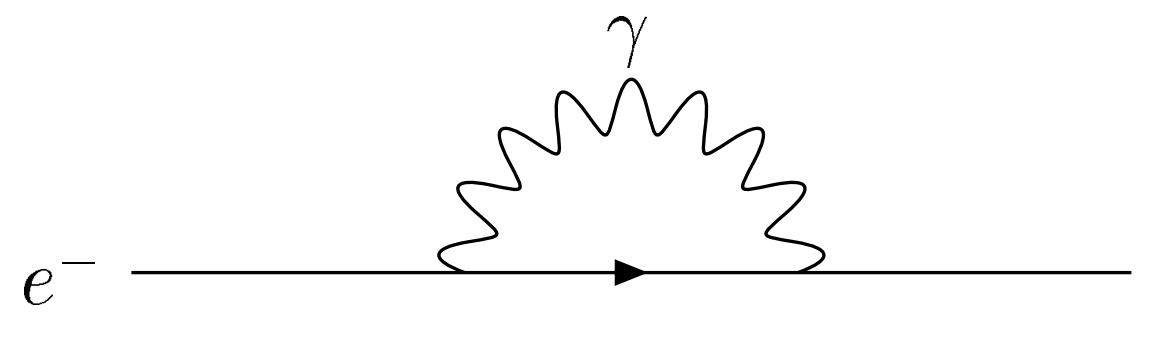
\includegraphics[width=7cm]{electronSelfE.png}
    \caption{The electron self energy. Figure from \cite{SusyHiggsSelfE}}
    \label{electronSelfE}
\end{figure}

A similar situation is observed in ferromagnets. At temperatures near $0$ K, a ferromagnet has a spin expectation value on the order of the atomic parameters. An experimenter can finely adjust the temperature until the system reaches a point where the spin expectation value is much smaller then the value predicted by atomic parameters. In this situation, there is no problem because an experimenter was adjusting the parameters, but there is no experimenter "fine tuning"\footnote{Sometimes this problem is referred to as a fine tuning problem for this reason. It is also called a naturalness problem, because the principle of naturalness states that all parameters should be of the same order} the radiative corrections to the Higgs mass \cite{Peskin}. This is why the Higgs self-coupling divergence "feels" wrong and motivates the need for a more complete theory.

Many theories beyond the standard model address this problem, but in doing so predict new particles. One such theory is Supersymmetry, which predicts that each standard model particle has a higher mass super partner. The minimal version of supersymmetry predicts particles that should have already been discovered at particle colliders prompting the rise of alternative theories. The next chapter discusses a type of particle that arises in some of these theories.

